
%***********************************************************************

% This is a template to be used for the preparation of
% papers submitted to the 33rd International Workshop on
% Statistical Modelling, to be held in Groningen, Netherlands,
% July 15-20, 2018.

% Please follow the following general guidelines:
%
% (1) Do not specify any definitions, commands or style parameters.
%     Upon submission, your file will be checked for presence of
%     \newcommand or \def statements and if found, error message will be reported
%     by the submission form.
%
% (2) Follow the template below very tightly.
%
% (3) Include .pdf figures using the \includegraphics
%      command, an example of which are given below.
%
% (4) Use file names which begin with the surname of the first author.
%
% (5) When creating labels for cross-references, please start always
%     by surname of the first author, e.g., \label{smith:likelihood}
%
% (6) The template below contains some example materials
%      to guide you through the preparation of your paper.  However,
%      remove all the redundant material from your final document
%      before submitting.

% The guidelines above are needed in order to be able to combine all
% the papers into a single proceedings book of acceptable quality.
% Please follow the guidelines as strictly as possible. Deviations may
% result in papers being either refused by the registration form
% or sent back to the authors with the request to change
% their documents according to the guidelines.

% Special characters:
% Please do not use special characters (e.g., accents).
% Use TeX composition instead, such as \~n, \'a, \`e, \v{s}, \r{u} etc.

% Changes as of IWSM 2013:
%  * \usepackage{booktabs} added which allows \toprule et al. in the tabular environment
%    (\hline\hline is not longer used)
%  * '^\T' added in iwsm.sty to denote transposed vectors and matrices within math (see example below)
%  * \usepackage{amsmath, amssymb} introduced since IWSM 2012 is allowed (allowing usage of boldsymbols
%    and other handy constructions (align, pmatrix etc.) within math)
%  * \usepackage{psfrag} introduced since IWSM 2012 is NOT allowed
%
%

%***********************************************************************
% PLEASE LEAVE THIS PART UNCHANGED
%***********************************************************************

\documentclass[twoside]{report}
\usepackage{iwsm}
\usepackage{graphicx}
\usepackage{amsmath, amssymb}
\usepackage{booktabs}

% Please do not specify any new definitions, any new commands,
% and do not specify any style parameters.
% The preamble of the document should be left unchanged.

% proofreading
\usepackage[textsize=scriptsize, backgroundcolor=lightgray, draft]{todonotes}
% ab todo note definition
\newcounter{todocounter}
\newcommand{\abtodo}[1]{
  \stepcounter{todocounter}\todo[color=black!30]{
    \textbf{AB[\thetodocounter]: }#1
  }
}

\begin{document}

%***********************************************************************
% PLEASE INSERT YOUR CONTENT FROM HERE
%***********************************************************************

% Title and running title to be used as left header:
\title{KOALA: Estimating coalition probabilities in multi-party electoral systems}
\titlerunning{Short title used as left header}

% Authors and running list of authors to be used as right header:
\author{Alexander Bauer\inst{1}, Andreas Bender\inst{1}, Andr\'e Klima\inst{1}, Helmut K\"{u}chenhoff\inst{1}}
\authorrunning{Bauer et al.}    %% use \authorrunning{Surname 1} if only 1 author
                                    %% use \authorrunning{Surname 1 and Surname2} if two authors
                                    %% use \authorrunning{Surname 1 et al.} if more than two authors

% Institutes of all authors
% Include city and country of each institute, do not include the full address.
\institute{Department of Statistics, Ludwig-Maximilians-Universit\"{a}t, Munich, Germany}

% E-mail of presenting author for correspondence
\email{Alexander.Bauer@stat.uni-muenchen.de}

% Brief abstract of the paper:
\abstract{
\abtodo{Ich würde vll. plakativer Anfangen: Übliche Berichterstattung bzgl. Wahlumfragen ist meist irreführend, weil ... Deshalb entwickelten wir ....}
We present a survey-based approach for the estimation of probabilities for specific coalition majorities in multi-party electoral systems. A Bayesian Multinomial-Dirichlet model with Monte Carlo simulation is used for estimation. The method is based on opinion polls conducted by established pollster institutes and is accompanied by a pooling approach to summarize multiple current surveys, accounting for dependencies between institutes.
%Potential biases of specific pollsters are not taken into account.
The method estimates sample uncertainty-based probabilities, if the election was held today. An implementation of the method in \texttt{R} is freely available.
}

% Keywords (at most 5):
\keywords{Election analysis; Opinion polls; Election reporting; Multinomial-Dirichlet; Pooling.}

% Produce the title:
\maketitle

%***********************************************************************

% Sections and subsections (do not use lower levels):

\section{Introduction and data}
Election polls as surveys conducted by different pollster institutes
\abtodo{``pollster instiute'' ist glaube ich ziemlich denglisch. Man sagt
denke ich survey institutes oder pollsters}
try to represent the public opinion based on a finite sample. Current reporting
on such surveys is most often limited to the observed shares, while sample uncertainty is usually ignored (cf. QUELLE).
\abtodo{Es wäre ganz gut hier konkrete Beispiele zu bringen, sonst hängt das Ganze
etwas in der Luft}
In our opinion, the focus in survey reporting in multi-party electoral systems should be shifted towards the most relevant question, i.e., how probable is a majority for a specific coalition.
We present our KOALA (Coalition Analysis) approach to estimate such probabilities
to bring more value to opinion poll-based reporting.

As database, we use opinion polls conducted by established pollster institutes,
quantifying the electoral behavior \textit{if an election was held today}.
Our approach is to be differentiated from prediction-aimed methods (cf. POLLYVOTE or NORPOTH \& GSCHWEND, 2010). We focus on the question of quantifying \textit{current} majority situations, not taking into consideration potential shifts until election
day.

A Bayesian Multinomial-Dirichlet model with Monte Carlo simulations is used for estimation. Also, a pooling approach is presented to summarize the results of multiple current opinion polls to reduce sample uncertainty.

All methods were implemented in \texttt{R} and are available in the open-source
package \texttt{coalitions} on GitHub (Bender \& Bauer, 2018). Also, an
interactive \texttt{shiny} app, hosted \texttt{koala.stat.uni-muenchen.de}
visualizes estimated coalition probabilities and is used to communicate the
results to the general public (QUELLE).


\section{Pooling approach}
\abtodo{Ich finde der Fokus liegt zu sehr auf dem Pooling. Ich würde in der
ersten Section nach der Intro zunächst die Hauptmethodik erklären ausgehend von
einem gegebenen Survey und dann zum Pooling überleiten.}
In the presence of multiple published opinion polls, pooling is used to summarize the observed results in order to reduce sample uncertainty. To assure a reliable pooling regarding the current public opinion, we only use polls published within the past 14 days and only use the most recent survey published by each pollster institute.

% Looking at a single poll $i$, the observed number of votes $X_j$ for each of $k$ parties follow a multinomial distribution with sample size $n_i$ and underlying, unknown party shares $\theta_j$ in the population:
% $$
% X_1,\ldots, X_k \sim Multinomial(n_i,\theta_1,\ldots,\theta_k).
% $$
Based on the multinomial distribution of the voter number $X_{ij}$ of party $j$ in poll $i$ with underlying true party share $\theta_j$, pooling over multiple polls representing independent random samples would lead to a multinomial distribution for the summed number of votes $\sum\limits_i X_{ij}$:
$$
\sum\limits_i X_{i1},\ldots, \sum\limits_i X_{ik} \sim Multinomial(\sum\limits_i n_i,\theta_1,\ldots,\theta_k).
$$

Further investigations however show that polls published by the main German
pollster institutes show a certain amount of correlation and the assumption of
independence does not hold. To account for this, we adjust the resulting
multinomial distribution by using an \textit{effective sample size} (cf. QUELLE).
Quantification of pairwise correlation is done based on the variance of the
difference between two polls. The following equation holds for two independent
random sample polls $A$ and $B$:

$$
\begin{aligned}
%Var(X_A - X_B) &= Var(X_A) + Var(X_B) - 2 \cdot Cov(X_A, X_B) \\
\Leftrightarrow Cov(X_{Aj}, X_{Bj}) &= \frac{1}{2} \cdot \left(Var(X_{Aj}) + Var(X_{Bj}) - Var(X_{Aj} - X_{Bj}) \right).
\end{aligned}
$$

We take $Var(X_{Aj})$ and $Var(X_{Bj})$ as the theoretical variances of the binomially distributed, observed voter numbers and estimate $Var(X_{Aj} - X_{Bj})$ based on the observed differences between the party shares. Having done so, one can estimate the covariance $Cov(X_{Aj}, X_{Bj})$ and accordingly also the correlation. As the binomial distribution is directly proportional to the sample size, the effective sample size $n_{\text{eff}}$ can be defined as the ratio between the estimated variance for the pooled sample and the theoretical variance of a sample of size one:
$$
n_{\text{eff}} = \frac{Var(\text{pooled})}{Var(\text{sample of size 1})},
$$
with, in the case of two surveys,
$$
Var(\text{pooled}) = Var(X_A + X_B) = Var(X_A) + Var(X_B) + 2 Cov(X_A,X_B)
$$
and $Var(\text{sample of size 1})$ the theoretical variance of the pooled share.

Looking at the party-specific correlations between 20 surveys conducted by the two most regular German pollster institutes, Emnid and Forsa, we on average end up with a medium high correlation, using mean party shares and sample sizes per institute for the theoretical variances. Other institute comparisons were not performed as too few surveys were conducted over comparable time frames. For simplicity, we set the correlation used in our methodology to $0.5$. For calculating $n_{\text{eff}}$ we base the calculation on the result of the biggest party, as the specific party choice only marginally affects $n_{\text{eff}}$.



\section{Calculation of probabilities}
\abtodo{Würde den Teil etwas ausführlicher machen, ggf. mit konkretem Beispiel
mit Tabelle der Umfrage und den sich daraus Ergebenden Wskten.}
For estimating probabilities for specific coalitions, we choose a Multinomial-Dirichlet model with an uninformative prior for the true party shares $\theta_j$ (QUELLE):
$$
\begin{aligned}
\boldmath{\theta} &= (\theta_1,\ldots,\theta_k)^\T \sim Dirichlet(\alpha_1,\ldots,\alpha_k), \\
\text{with} &\ \ \ \ \ \ \ \ \ \ \ \ \ \ \ \alpha_1 = \ldots = \alpha_k = \frac{1}{2}
\end{aligned}
$$
Basing the Bayesian model on one (pooled) survey the posterior also results in a Dirichlet distribution with parameters $\alpha_j = x_j + \frac{1}{2}$ for each party $j$.

Probabilities for specific events can now be estimated using Monte Carlo simulations of random election outcomes. After calculating to which effective number of seats in parliament the simulated results lead, one can easily calculate probabilities by taking the share of times some specified event occurs. To adjust for observed survey shares generally being only published as rounded numbers, before applying the Bayesian model we add uniformly distributed random noise $r_\gamma \sim U[-\gamma,\gamma]$ to the
shares (e.g., $\gamma = 0.5\%$) and rescale the sum to $100\%$.

\begin{figure}[!ht]\centering
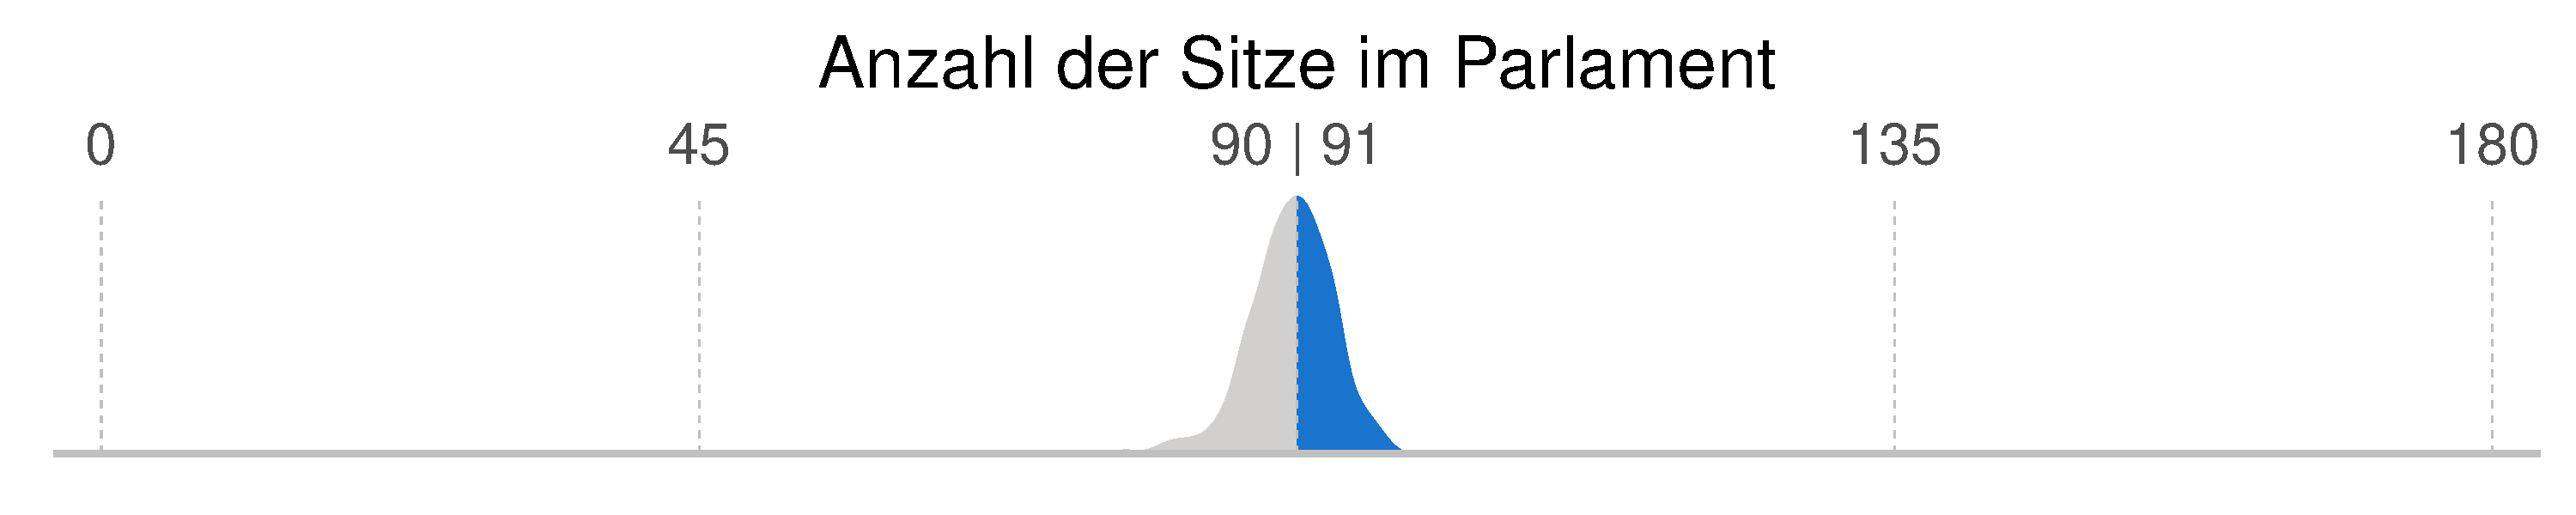
\includegraphics[width=\textwidth]{figures/bauer_seatDist.pdf}
\caption{\label{bauer:dens} Density of $1,000$ simulated shares of parliament seats for the coalition CSU/FDP in the Bavarian state election. The blue area marks simulations with a majority.}
\end{figure}
\abtodo{Denke man kann hier coolere Grafik einfügen. z.B. die
Density-Verläufe von Schwarz-Gelb die in Spectrum verwendet wurde. Siehe
z.B. https://gist.github.com/adibender/28041453a2a8c3e42c09484a55668d55}

For visualizing the probability together with underlying uncertainty for a specific coalition majority we recommend using a density plot as shown in Figure~\ref{bauer:dens}.


\section{Conclusion}
We presented an approach to estimate probabilities for specific election outcomes based on publicly available opinion polls. Pooling allows for the inclusion of information from multiple surveys. Visualizing the results on a publicly available website for chosen elections, our long-term goal is to make proper uncertainty assessment standard in general opinion poll-based reporting.


%***********************************************************************

% Acknowledgments, if needed:
\acknowledgments{Special Thanks to ... }

%***********************************************************************

% References should be placed in the text in author (year) form.
% The list of references should be placed below IN ALPHABETICAL ORDER.
% (Please follow the format of the examples very tightly).

\references
\begin{description}
\item[Bender, A. and Bauer, A.] (2018).
{\it adibender/coalitions (Version v0.5.7).}
Zenodo. \texttt{http://doi.org/10.5281/zenodo.1172595}
\item[Diggle, P.J., Liang, K-Y., and Zeger, S.L.] (1994).
     {\it Analysis of Longitudinal Data}.
     Oxford: Clarendon Press.
\item[Green, P.J. and Silverman, B.W.] (1994).
     {\it Nonparametric Regression and Generalized Linear Models}.
     London: Chapman \& Hall.
\item[Henderson, C.R.] (1973).
     Sire evaluation and genetic trends.
     In: {\it Proceedings of the Animal Breeding and Genetics Symposium in
     Honour of Dr.\ L.\ Lush}, Champaign, Illinois, 10\,--\,41.
\item[Lee, Y. and Nelder, J.A.] (1996).
     Hierarchical generalized linear models.
     {\it Journal of the Royal Statistical Society, Series B}, {\bf 58},
      619\,--\,678.
\item[Robinson, G.K.] (1991).
     That BLUP is a good thing: the estimation of random effects (with Discussion).
     {\it Statistical Science}, {\bf 6}, 15\,--\,51.
\end{description}

\end{document}
